%% 
%% Copyright 2007-2020 Elsevier Ltd
%% 
%% This file is part of the 'Elsarticle Bundle'.
%% ---------------------------------------------
%% 
%% It may be distributed under the conditions of the LaTeX Project Public
%% License, either version 1.2 of this license or (at your option) any
%% later version.  The latest version of this license is in
%%    http://www.latex-project.org/lppl.txt
%% and version 1.2 or later is part of all distributions of LaTeX
%% version 1999/12/01 or later.
%% 
%% The list of all files belonging to the 'Elsarticle Bundle' is
%% given in the file `manifest.txt'.
%% 
%% Template article for Elsevier's document class `elsarticle'
%% with harvard style bibliographic references

\documentclass[preprint,review,12pt,authoryear]{elsarticle}

%% Use the option review to obtain double line spacing
%% \documentclass[authoryear,preprint,review,12pt]{elsarticle}

%% Use the options 1p,twocolumn; 3p; 3p,twocolumn; 5p; or 5p,twocolumn
%% for a journal layout:
%% \documentclass[final,1p,times,authoryear]{elsarticle}
%% \documentclass[final,1p,times,twocolumn,authoryear]{elsarticle}
%% \documentclass[final,3p,times,authoryear]{elsarticle}
%% \documentclass[final,3p,times,twocolumn,authoryear]{elsarticle}
%% \documentclass[final,5p,times,authoryear]{elsarticle}
%% \documentclass[final,5p,times,twocolumn,authoryear]{elsarticle}

%% For including figures, graphicx.sty has been loaded in
%% elsarticle.cls. If you prefer to use the old commands
%% please give \usepackage{epsfig}

%% The amssymb package provides various useful mathematical symbols
\usepackage{amssymb}
%% The amsthm package provides extended theorem environments
\usepackage{amsthm}
\usepackage{amsmath}
\usepackage {caption}
% \renewcommand{\figurename}{\textbf{Fig}}
% \captionsetup[figure]{labelsep=period}

%% The lineno packages adds line numbers. Start line numbering with
%% \begin{linenumbers}, end it with \end{linenumbers}. Or switch it on
%% for the whole article with \linenumbers.
%% \usepackage{lineno}

\journal{Journal of the Mechanics and Physics of Solids}

\begin{document}
\captionsetup[figure]{name={\textbf{Fig.}},labelsep=period} 


\begin{frontmatter}

%% Title, authors and addresses

%% use the tnoteref command within \title for footnotes;
%% use the tnotetext command for theassociated footnote;
%% use the fnref command within \author or \affiliation for footnotes;
%% use the fntext command for theassociated footnote;
%% use the corref command within \author for corresponding author footnotes;
%% use the cortext command for theassociated footnote;
%% use the ead command for the email address,
%% and the form \ead[url] for the home page:
%% \title{Title\tnoteref{label1}}
%% \tnotetext[label1]{}
%% \author{Name\corref{cor1}\fnref{label2}}
%% \ead{email address}
%% \ead[url]{home page}
%% \fntext[label2]{}
%% \cortext[cor1]{}
%% \affiliation{organization={},
%%            addressline={}, 
%%            city={},
%%            postcode={}, 
%%            state={},
%%            country={}}
%% \fntext[label3]{}

\title{Inverse design workflow of implicit surface-based cellular materials via conditional generative model and active Learning}


\author[1]{Jiaxuan Ma}
\author[3]{Bin Cao}
\author[1]{Yuan Tian, \corref{cor1}}
\ead{tian0321@shu.edu.cn}
\author[1,2]{Sheng Sun, \corref{cor1}}
\ead{mgissh@t.shu.edu.cn}


\address[1]{Materials Genome Institute, Shanghai University, Shanghai, 200444, China}
\address[2]{Shanghai Frontier Science Center of Mechanoinformatics, Shanghai University, Shanghai, 200444, China}
\address[3]{Advanced Materials Thrust, Hong Kong University of Science and Technology (Guangzhou), Guangzhou, 511400, Guangdong, China}

\cortext[cor1]{Corresponding author}

\begin{abstract}
Implicit surface-based cellular materials have gained widespread adoption in bone scaffolds applications due to their similarities to bone structure. These materials excel in providing good mechanical properties and bioadaptability, creating suitable conditions for bone tissue regeneration. However, the rational design of these materials typically depends on prior knowledge of experts and requires large of  trail-and-error experiments. Here, we present a data-efficient two-stage bi-objective optimization method within a machine learning framework that considers the varying costs associated different objectives. Specifically, we employ this methodology to orthopedic implant inverse design, integrating generative model, active leaning, and finite element analysis to achieve both biocompatible elastic modulus and higher yield strength cellular materials. Our approach demonstrates remarkable improvements in overall performance compared to initial datasets, while simultaneously reducing about sixfold design cost relative to one-step bi-objective optimization machine learning method. This methodology establishes an efficient paradigm for the rapid and intelligent design of cellular materials with tailored mechanical properties, particularly valuable in scenarios involving objectives with unbalanced computational costs.
\end{abstract}

%%Graphical abstract
\begin{graphicalabstract}
%\includegraphics{grabs}
\end{graphicalabstract}

%%Research highlights
\begin{highlights}
\item Developing TPMS-GAN with navigator was proposed to generate TMPS unit cell under desired conditions of mechanical properties and geometries.
\item Developing Inversed TPMS-GAN to design TPMS unit cell in geomety feature in a explainable way instead of through latent space or coefficients of implicit function 
\item Proposing a constraint-aware active learning method to address bi-objective optimization problem with unbalanced costs of objective function. 
\end{highlights}

\begin{keyword}

Multi-objective optimization \sep Cellular structure design \sep Generative adversarial network \sep Constraint-aware active learning
\end{keyword}

\end{frontmatter}

%% \linenumbers

%% main text
\section{Introduction}
Cellular materials are one of the most widely adopted engineering materials due to their excellent mechanical performance and adaptable properties, such as lightweight structures \citep{Schaedler2011, Berger2017, Han2015, Tancogne-Dejean2018}, thermal insulation \citep{Li2021d}, acoustic \citep{Sekar2024} and tissue engineering \citep{Li2024c,Peng2023,Tabrizian2024}. Moreover,  recent progress in additive manufacturing (AM) has further enabled the inexpensive and tailored fabrication of complex structures. Despite the broad applicability and immense potential of cellular materials, designing them is particularly difficult.

The traditional approach to design often relies on nature-inspired structures \citep{Fernandes2021,Bandyopadhyay2021,Sethi2023}, human intuition \citep{Schaedler2011,Berger2017,Xu2016a}, and numerical simulations, including topology optimization \citep{Andersen2019,Bendsoe1999,Collet2018}, spinodal separation \citep{Hsieh2019,Roding2022}, or Gaussian random fields \citep{Kumar2020,Zheng2020abc}. These rule-based methods are typically exhausting and time-consuming. Furthermore, the performance of resultant designs is highly dependent on the professional expertise of the designer.
 
With the rapid development of artificial intelligence (AI), machine learning has significantly transformed the design paradigm of cellular materials. By learning from data, machine learning models can effectively capture the non-linear relationships between geometric features and mechanical properties of cellular materials. Once trained, these models offer a low-cost inference capability, serving as surrogates for expensive numerical simulations and experiments. Consequently, machine learning models can be seamlessly integrated into heuristic algorithms facilitating the optimization of cellular material structures with target mechanical properties, such as elastic modulus \citep{Garland2021,Lee2022,Chen2024b}, bulk resistance \citep{Liu2020a}, and stress-strain curve \citep{Deng2022a,Ma2020b}.  However, surrogate optimization is a high-throughput selection process that necessitates multiple invocations of machine learning models, presenting challenges for global optimization problems and real-time design requirements.

Generative models, such as variational auto-encoder (VAE) \citep{Wang2020a,Zheng2023},  generative adversarial network (GAN) \citep{Nie2020, Shen2022,Kim2020b} and diffusion model \citep{Bastek2023,Maze2022,Vlassis2023}, have demonstrated significant capabilities in cellular materials design. These models can learn the distribution of structures of training dataset and sample new structures from it. In particular, conditional generative models can produce novel structures with a target property, making them suitable for inverse design problems in cellular materials where multiple structures correspond to a single property. Although generative models have been widely used in designing cellular materials, the cost of building dataset has rarely been considered, especially in multi-objective problems. It is common to encounter the scenario where one objective function is inexpensive while another is costly. This is particularly prevalent in design of cellular structures, where linear and nonlinear mechanical properties must be considered simultaneously.

Triply periodic minimal surfaces (TPMS) are a family of cellular materials based on implicit functions, and the shapes of the unit cells can be controlled by adjusting the coefficients of the implicit function and the constants of the level set \citep{Ma2020a}. TPMS are characterized by their locally symmetric saddles shapes with vanishing mean curvature and non-positive Gaussian curvature. Each domain of TPMS is a single, connected, infinite component without sealed cavities in its geometry \citep{Kapfer2011}. These structures are particularly valuable in orthopedic implants due to their ability to mimic the diverse characteristics of bone. For such applications, it is crucial that the elastic module of the implant matches that of human bone to minimize stress shielding, while the yield stress should be as high as possible to provide adequate mechanical support and a long fatigue life. The elastic modulus of TPMS unit cell can be readily evaluated using numerical homogenization methods. However, the evaluation of yield stress incurs significant costs due to the nonlinear plasticity constitute of base materials via finite element method (FEM).

In the work, we propose a two-step strategy that integrates generative model with active learning algorithms to address bi-objective design problem of TPMS unit cells associated with imbalanced costs of properties. As demonstrated in Fig \ref{fig:1}, our approach consists of three main parts: (1) generate structures with a desired elastic modulus. In this step, a TPMS-GAN model is trained on a dataset containing TPMS unit cells and their corresponding elastic modulus. Then the generator of the TPMS-GAN produces structures with target elastic modulus, forming a virtual structure space (VSS). (2) inversed TPMS-GAN (ITPMS-GAN) model was developed to explore the latent space of TPMS-GAN, allowing for direct geometric manipulation of TPMS structures instead of modifying implicit function parameters. (3) an elastic modulus constraint-aware active learning approach for yield strength optimization. Initially, the yield strength of a select number of TPMS structures within VSS are evaluated to establish the initial dataset via FEM. Subsequently, elastic modulus constraint-aware active learning based on Bayesian optimization (BO) is employed to optimize the yield strength of TPMS unit cells. BO method has been proven significant efficiency in materials design with small data \citep{Ma2024b,Cao2024a,Tian2024a}.

\begin{figure}
    \centering
    \includegraphics[width=1\linewidth]{figures/1.pdf}
    \caption{\textbf{An overview of the proposed workflow for TPMS unit cells design.} \textbf{a} The generator in TPMS-GAN model produces virtual design space ($\Omega_E$) with desired elastic modulus. \textbf{b} The ITPMS-GAN model was developed to edit the TPMS structure through geometry features to rich diversity of candidates in $\Omega_E$. \textbf{c} The machine learning (ML) algorithm interactively queries the FEM to discovery new TPMS designs with high yield strength and target elastic modulus through constrained active learning in $\Omega_E$.}
    \label{fig:1}
\end{figure}

\section{Models and methods}

\subsection{TPMS-based cellular structures}

TPMS can be produced by a simple level-set approximation equation from a sum defined in terms of the Fourier series \citep{Gandy2001,Al-Ketan2019}:
\begin{equation}
 \Psi(\boldsymbol{r})=\sum_kF(\boldsymbol{k})\text{cos}([2\pi \boldsymbol{k}\cdot \boldsymbol{r}-\alpha(\boldsymbol{k})])=0
\label{eq:1}
\end{equation}
where $\boldsymbol{k}$ is the reciprocal vector, $\alpha(\boldsymbol{k})$ is a phase shift, and the structure $F(\boldsymbol{k})$ is an amplitude associated with the given $\boldsymbol{k}$ vector. Truncating the series to the leading term gives rise to a function $\phi$ that consists of a combination of trigonometric functions and satisfies the equality $\phi(x,y,z)=c$. The function $\phi(x, y, z)$ defines a surface evaluated at the isovalue (i.e., level-set constant) $c$ and has a topology similar to that of a minimal surface. 

\subsection{Effective properties of homogenized cellular structures}
\label{subsec:homo}

In the work, a voxel-based asymptotic homogenization method \citep{Dong2019} is employed to calculate the effective elastic tensor of TPMS unit cells. The asymptotic homogenization method posits that physical quantities such as stress and strain depend on both the macroscale ($X$) and the microscale ($x/\varepsilon$), where $\varepsilon$ is the scale factor. These quantities are homogenized at the macroscale and exhibit periodicity at the microscale. The microscopic strain tensor can be asymptotically expanded, and by neglecting higher-order terms, it can be expressed as:
\begin{equation}
    \varepsilon = \bar{\varepsilon} + \varepsilon^{*}
\label{eq:2}
\end{equation}
Here, $\bar{\varepsilon}$ represents the mean or macroscopic strain within the unit cell, while $\varepsilon^{*}$ denotes the perturbation strain at the periodic microscale. The perturbation strain is derived from the mechanical balance equation:
\begin{equation}
\int_{\Omega}\hat{\varepsilon}^T:\mathbb{C}:\varepsilon^{*}d\Omega = \int_{\Omega}\hat{\varepsilon}^T:\mathbb{C}:\bar{\varepsilon}
\label{eq:3}
\end{equation}
In this equation, $\hat{\varepsilon}$ is the virtual strain, $\mathbb{C}$ is the elastic tensor of the constituent materials, and $\Omega$ represents the unit cell. This equation is numerically discretized and evaluated using the FEM, which employs eight-node hexahedrons to voxelize each unit cell into $40 \times 40 \times 40$ cubes (more details are provided in Supplement S1). Once $\varepsilon^{*}$ is obtained, the effective elastic tensor $\mathbb{C}^H$ can be determined using the following equation:
\begin{equation}
\mathbb{C}^H:\bar{\varepsilon} = \frac{1}{|\Omega|}\int_{\Omega}\mathbb{C}:(\bar{\varepsilon}+\varepsilon^{*})d\Omega
    \label{eq:4}
\end{equation}
where $|\Omega|$ denotes the volume of the unit cell.

From the effective elastic tensor $\mathbb{C}^H$, the compliance tensor $\mathbb{S}^H$ can be derived, and its Voigt form is expressed as:
\begin{equation}
\mathbb{S}^H = \begin{bmatrix}
\frac{1}{E_x} & -\frac{v_{yx}}{E_y} & -\frac{v_{zx}}{E_z} & 0 & 0 & 0 \\
-\frac{v_{xy}}{E_x} & \frac{1}{E_y} & -\frac{v_{zy}}{E_z} & 0 & 0 & 0 \\
-\frac{v_{xz}}{E_x} & -\frac{v_{yz}}{E_z} & \frac{1}{E_z} & 0 & 0 & 0 \\
0 & 0 & 0 & \frac{1}{G_{yz}} & 0 & 0 \\
0 & 0 & 0 & 0 & \frac{1}{G_{zx}} & 0 \\
0 & 0 & 0 & 0 & 0 & \frac{1}{G_{xy}}
\end{bmatrix}
\label{eq:5}
\end{equation}

In this matrix, $E_i$ represents the elastic modulus along the $i^{\text{th}}$ direction, where $i \in \{x, y, z\}$. In the work, for cubic symmetric unit cells, we have effective elastic module $E^H=E_x=E_y=E_z$. Additionally, elastic moduli in other directions can be obtained from $\mathbb{S}^H$ using the following equation:
\begin{equation}
\frac{1}{E_{ijk}} = \mathbb{S}^H_{11} - 2 \left(\mathbb{S}^H_{11} - \mathbb{S}^H_{12} - \frac{1}{2} \mathbb{S}^H_{44} \right) \times \left( \ell_{i1}^2 \ell_{j2}^2 + \ell_{j2}^2 \ell_{k3}^2 + \ell_{i1}^2 \ell_{k3}^2 \right)
    \label{eq:6}
\end{equation}
Here, $E_{ijk}$ is the elastic moduli along the $[i,j,k]$ direction, and $\ell$ is the cosine of the angle between the orientation $[i,j,k]$ and the coordinate axes $[x, y, z]$. This approach allows for the evaluation of elastic modulus in any orientation of the unit cell, facilitating the construction of a three-dimensional elastic modulus surface.

\subsection{The architecture of TPMS-WGAN model}

In the work, we employ a conditional Wasserstein GAN comprising four components: a generator network ($G_\phi$), a discriminator network ($D_\theta$),  a navigator network ($R_\omega$) and a condition module $\boldsymbol{C}$ that consists of mechanical properties and geometry characterization of the TPMS unit cell. Each condition can be turned on/off during the training process to meet various design requirements (see Fig.\ref{fig:3} ). The generator $G_\phi$ (with set of trainable parameters $\phi$) map the Gaussian noise ($z$) and conditions to TPMS's parameter space $\boldsymbol{p}$ in $\mathbb{R}^4$, and achieve the fake $\boldsymbol{p}'$. While the discriminator $D_\theta$ (with set of trainable parameters $\theta$) evaluate whether a given set of structure parameters are "real" or not. It takes $\boldsymbol{p},\boldsymbol{p}'$ and  $\boldsymbol{C}$ as input and its output $D_\theta(\boldsymbol{p}'|\boldsymbol{C})$ is a function value representing the degree of realism of $\boldsymbol{p}'$. During the training process, the goal of the generator $G_\phi$ is to produce structure parameters $\boldsymbol{p}'$ of TPMS that can deceive the discriminator $D_\theta$. Simultaneously, the objective of $D_\theta$ is to distinguish structures $\boldsymbol{p}'$ generated by $G_\phi(\boldsymbol{z}|\boldsymbol{C})$ and real structure $\boldsymbol{p}$. $G_\phi$ and $D_\theta$ play the following two-player minimax game with loss function:
\begin{equation}
\mathcal{L}_{(G_\phi, D_\theta)}= \min_G \max_{D} \mathbb{E}_{\boldsymbol{p} \sim \mathbb{P}_r} \left[ D_\theta(\boldsymbol{p}|\boldsymbol{C}) \right] - \mathbb{E}_{\boldsymbol{p}' \sim \mathbb{P}_g} \left[ D_\theta (\boldsymbol{p}') \right]
\label{eq:7}
\end{equation}
where $D$ belongs to the set of 1-Lipschitz functions, $\mathbb{P}_r$ and $\mathbb{P}_g$ are distribution of dataset and model distribution implicitly defined by $\boldsymbol{p}'=G_\phi(\boldsymbol{z}|\boldsymbol{C}) $, respectively. In addition, we employ the Wasserstein GAN gradient penalty (WGAN-GP) method to address the delicate and unstable training issues associated with vanishing or exploding gradients. Further details can be found in \citep{Gulrajani2017}.

\begin{figure}
    \centering
    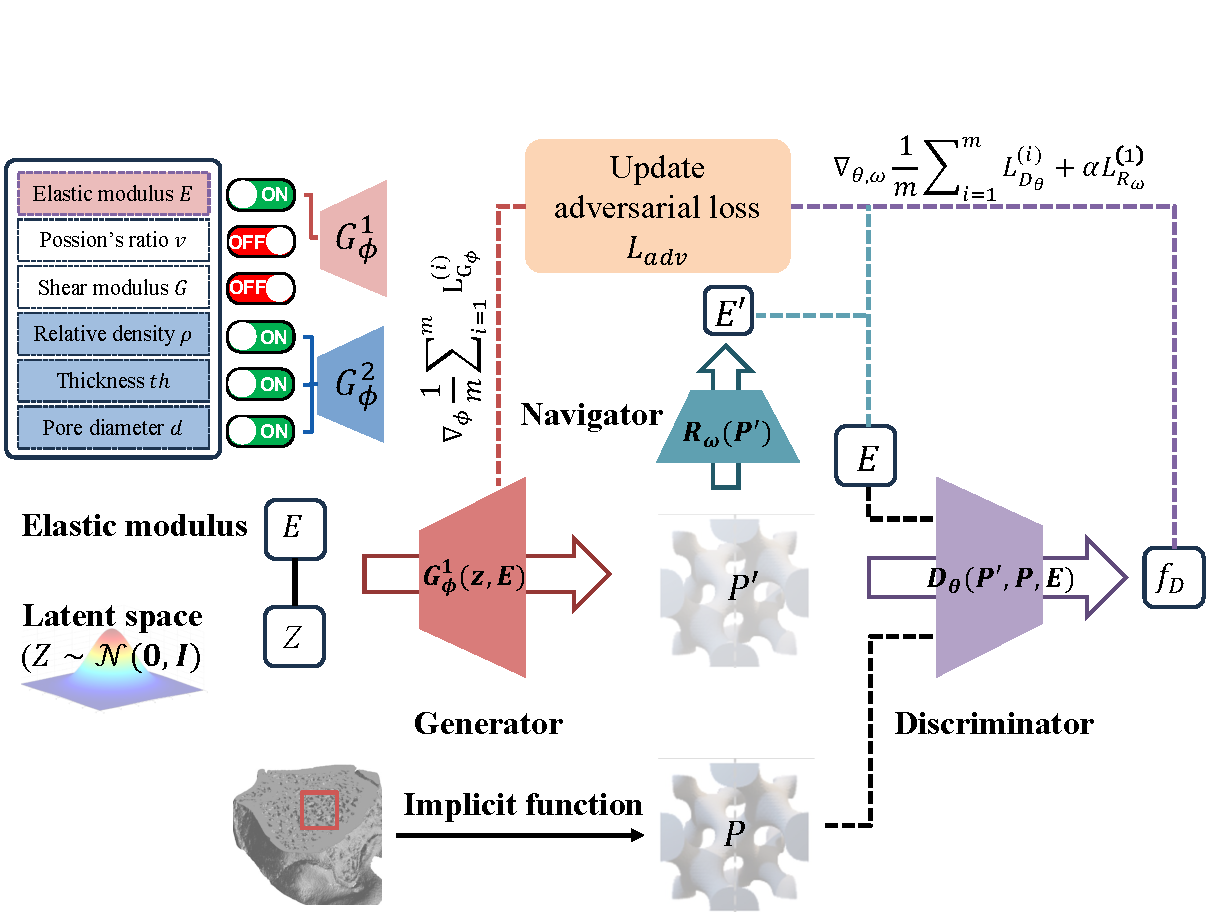
\includegraphics[width=1\linewidth]{figures/3.pdf}        
    \caption{\textbf{Generative modeling framework}. The conditional WGAN model can address multiple conditions including property and geometry characterizations of TPMS unit cell, here we called it TPMS-WGAN. Each condition can be turned on$/$off to meet various design requirements. Considering elastic modulus, the TPMS-WGAN takes effective elastic modulus $E$ and random noise $\boldsymbol{z} (\boldsymbol{z}\sim\mathcal{N}(\mathbf{0},\mathbf{I})$,a Gaussian distribution of zero mean and the identity as the covariance matrix) as input to generator $G_\phi^1$, and the generated TPMS structure (denoted by implicit function parameters $\boldsymbol{p}'$), $E$ and the real TPMS structure (denoted by $\boldsymbol{p}$) are then passed to the discriminator $D_\theta$ to output value $f_D$. The $\boldsymbol{p}'$ also is passed navigator $R_\omega$ to obtained the predicted effective elastic modulus $E'$.}
    \label{fig:3}
\end{figure}
  
\subsection{Constraint-aware active learning}
\label{sec:2-4}
Active learning methods based BO are popular in addressing black-box problems that are expensive to evaluate. Unlike gradient-based and heuristic optimization techniques, which rely solely on the predicted values of surrogate models, BO utilizes the probabilistic predictions of a surrogate model that is updated sequentially. BO comprises two primary components: the surrogate model and the acquisition function (AF). Surrogate model make it possible to search the virtual design space at low computational costs with uncertainty, while AF is employed to evaluate the score of samples in a given virtual design space, considering exploration and exploitation. In the work, support vector machine (SVM) model is used to surrogates the expensive objective i.e., the FE calculation of yield stress of the TPMS unit cell. Then bootstrap method is utilized to introduce the prediction uncertainties to build the probability model $y=f(\boldsymbol{x})+\varepsilon$. The probability model is directly applied to estimate the mean value ($\mu$) and associated uncertainties ($\Sigma^2$) of candidates in a unexplored virtual design space.

BO is a sequential optimization process that explore the optimal solution through iteration. At each iteration, the SVM model is used to evaluate all the unobserved sample within virtual design space, and select the most promising candidate $\hat{\boldsymbol{x}}^*$ for simulation or experiment to obtain $f(\hat{\boldsymbol{x}}^*)$ according to AF. The obtained new data pair $(\hat{\boldsymbol{x}}^*, f(\hat{\boldsymbol{x}}^*))$ is added to the known data set $\mathcal{D} = \{(\boldsymbol{x}_1, f(\boldsymbol{x}_1)), \ldots, (\boldsymbol{x}_n, f(\boldsymbol{x}_n))\}$ and update SVM to enhance its prediction ability. The process is repeated iteratively until a predefined convergence criterion or budget is satisfied. The critical step is the selection of candidate point $\hat{\boldsymbol{x}}^*$ which is done via an AF that enables active learning of the objective $f(\cdot)$\citep{Settles2009ActiveLL}. AFs are denoted by the expected value of a user-defined utility function conditioned on the available data $\mathcal{D}$:
\begin{equation}
    \alpha(\boldsymbol{x}) = \mathbb{E}[I(\boldsymbol{x})|\mathcal{D}]
\label{eq:8}
\end{equation}
A popular utility function is expected improvement (EI) which rewards the large improvement over the best observed value $f^*$ in $\mathcal{D}$ (evaluated thus far), that is:
\begin{equation}
    I_\text{EI}(\boldsymbol{x})=\text{max}(f(\hat{\boldsymbol{x}})-f^*, 0)
    \label{eq:9}
\end{equation}
The corresponding AF can now by obtained by substituting Eq. \ref{eq:9} in Eq. \ref{eq:8} and using the reparametrization trick (more details are provided in Supplementaty S2):
\begin{equation}
\alpha_\text{EI}(\boldsymbol{x}) = \left(\mu(\boldsymbol{x}) - f^*\right) \Phi\left(\frac{\mu(\boldsymbol{x}) - f^*}{\Sigma(\boldsymbol{x})}\right) + \Sigma(\boldsymbol{x}) \phi\left(\frac{\mu(\boldsymbol{x}) - f^*}{\Sigma(\boldsymbol{x})}\right)
\label{eq:10}
\end{equation}
where $\phi(\cdot)$ is the probability density function (PDF), $\Phi(z)$ is the cumulative density function (CDF) of the standard normal random variable $z$.
The first term on the right-hand side addresses exploitation, while the second term is associated with exploration. The AF is employed to score the unknown samples in virtual design space, guiding the selection of potential candidates for next simulation or experiments.

Adding inequality constraints to BO can be formed by
\begin{equation}
\max_{c(\boldsymbol{x}) \leq \lambda} f(\boldsymbol{x})
\label{eq:11}
\end{equation}
where $c(\boldsymbol{x})$ are the other results of data set $\mathcal{D}$, and it is modeled by another probability model similar to $f(\cdot)$. The $c(\boldsymbol{x})\leq \lambda$ is a constraint function that limited the feasible area in virtual design space. The constraint-aware EI for a candidate $\hat{\boldsymbol{x}}$ can be written by:
\begin{equation}
I_{\text{EI-C}}(\hat{\boldsymbol{x}})=\Delta_\text{C}(\hat{\boldsymbol{x}})\text{max}\{0, f(\hat{\boldsymbol{x}})-f^*\}=\Delta_\text{C}(\hat{\boldsymbol{x}})I_{\text{EI}}(\hat{\boldsymbol{x}})
    \label{eq:12}
\end{equation}
where $\Delta_\text{C}(\hat{\boldsymbol{x}})\in \{0,1\}$ is a feasibility indicator function that is 1 if $c(\hat{\boldsymbol{x}})\leq \lambda$, and 0 otherwise. 
The distribution of random variable $\Delta(\hat{\boldsymbol{x}})$ is Bernoulli distribution:
\begin{equation}
    PF(\hat{\boldsymbol{x}}):=Pr[c(\boldsymbol{x})\leq \lambda] 
    \label{eq:13}
\end{equation}
The quantity $PF(\hat{\boldsymbol{x}})$ is a cumulative distribution function. These steps lead to the  constraint-aware expected improvement AF:
\begin{equation}
\begin{aligned}
\alpha_{\text{EI-C}}(\hat{\boldsymbol{x}}) &=\mathbb{E}[I_\text{EI-C}(\hat{\boldsymbol{x}})]\\
&= \mathbb{E}[\Delta_{C}(\hat{\boldsymbol{x}})I_{\text{EI}}(\hat{\boldsymbol{x}})|\hat{\boldsymbol{x}}]\\
&= \mathbb{E}[\Delta_{C}(\hat{\boldsymbol{x}})|\hat{\boldsymbol{x}}]\mathbb{E}[I_\text{EI}(\hat{\boldsymbol{x}})|\hat{\boldsymbol{x}}]\\
&=PF(\hat{\boldsymbol{x}})\alpha_{\text{EI}}(\hat{\boldsymbol{x}})
\end{aligned}
\label{eq:14}
\end{equation}
Thus $\alpha_{\text{EI-C}}(\hat{\boldsymbol{x}})$ is the a standard EI of $\hat{\boldsymbol{x}}$ over the feasible point weighted by the probability that $\hat{\boldsymbol{x}}$ is feasible. In the work, we extend the constraint-aware expected improvement AF by surrogate $PF(\hat{\boldsymbol{x}})$ with the normalized distance between the constraint value $c(\hat{\boldsymbol{x}})$ within a virtual space and a target point $c^*$. This distance is mathematically expressed as $ND(||c(\hat{\boldsymbol{x}})-c^*||)$. By incorporating the constrained function, the distribution of \(\alpha_{\text{EI}}(\hat{\boldsymbol{x}})\) is adjusted point-by-point. Notably, this approach eliminates the need to construct an additional probability model to surrogate the constraint function $c(\hat{\boldsymbol{x}}) $. Consequently, Equation \ref{eq:17} can be reformulated as $\alpha_{\text{EI-C}}(\hat{\boldsymbol{x}}) =ND(||c(\hat{\boldsymbol{x}})-c^*||)\alpha_{\text{EI}}(\hat{\boldsymbol{x}})
$. 

Figure \ref{fig:6} schematically illustrates the comparison between the constraint-unaware active learning process and the constraint-aware active learning process. The optimal point in the constraint-unaware objective function is denoted by blue dot (Fig \ref{fig:6}a), while the optimal point in the constraint-aware objective function is denoted by red dot (Fig\ref{fig:6}b). We introduced a constraint function expressed by a normalized function to alters the EI score of candidates in a virtual data space, which is evident in the shift of the most promising point to query, as depicted from Fig. \ref{fig:6} c to Fig \ref{fig:6}d (more details about the toy problem are provided in Supplementary S3). The method can accurately found the optimal point in the constraint-aware objective function. Notably, the selection of the subsequent query point, whether driven by prediction (exploitation), uncertainty (exploration), or a trade-off between the two, will be influenced by the constraints. 

\section{Results and Discussions}

\subsection{Database of TPMS-based cellular structures }

The Shcoen's gyroid (G) and diamond (D) structures of TPMS present a highly versatile geometry with notably wide range of elastic modulus \citep{Lee2016}. The structures of G and D are defined through the following implicit functions $f(x,y,z)$:
\begin{equation}
\begin{aligned}
f_G(x,y,z)&= cos(2\pi y)sin(2\pi x)+cos(2\pi x)sin(2\pi z)\\&+cos(2\pi z)sin(2\pi y)+t_1 = 0, t_1 =0
\end{aligned}
\label{eq:15}
\end{equation}
\begin{equation}
\begin{aligned}
f_D(x,y,z)&=cos(2\pi x)cos(2\pi y)cos(2\pi z)\\&-sin(2\pi x)sin(2\pi y)sin(2\pi z)+t_2=0, t_2 =0
\end{aligned}
\label{eq:16}
\end{equation}
In addition to concise representation, TPMS-based cellular unit also can be diversified by combining several functions and adjusting corresponding coefficients \citep{Wang2019b}. In the work, the cellular structures are created as a combination of G and D structures, and the weight sum of their implicit functions are denoted by:
\begin{equation}
\begin{aligned}
    f_{Hybrid}(x, y, z) &=\alpha_1 (4f_G(x,y,z))+\alpha_2(4f_D(x, y,z ))\\
    \alpha_1+\alpha_2 &= 1,
    0\leq\alpha_1, \alpha_2 \leq1,
\end{aligned}
\label{eq:17}
\end{equation}
where $\alpha_1$ and $\alpha_2$ are randomized with a fixed sum of 1 to generated diverse cellular structures. The level set value $t_1$ and $t_2$ are limited in range from -0.5 to 0.5, which determine the volume fraction (i.e., relative density ) of a unit cell by thickening or thinning the surfaces. By varying the parameters $\alpha_1, \alpha_2, t_1, t_2$ in Eq.\ref{eq:4}, the TPMS structures can be adjusted, as illustrated in Fig\ref{fig:2}a. The merging operation not only produces geometric variations but also influences the mechanical properties of TPMS unit cells. 

We construct a rich database of TMPS unit cell by perturbing the parameters $\{\alpha_1, \alpha_2, t_1, t_2\} $ through Latin hyper-cube sampling (LHS) , resulting in 1372 unique structures (exclude some invalid structures). These structures exhibit orthotropic isotropic mechanical properties due to the cubic symmetric property of merged TPMS unit cell. For each structure, the effective mechanical stiffness tensor was computed by numerical homogenization method as illustrated in Section \ref{subsec:homo}. The mechanical properties of the cellular materials are influenced by both the scaffold architecture and the constituent materials. In the work, Ti6Al4V (Ti) was used as the constituent materials for orthopedic implants \citep{Peng2023} (material's parameters are provided in Supplementary S1). Ti alloy is bio-inert in human bodies and has been the de facto choice for 3D-printed orthopedic implants, achieving successful clinical applications in repairing bone defects. Figure \ref{fig:2}b shows the mechanical properties' distribution (effective elastic modulus $E$, Possion's ratio $v$) of G, D and Hybird TPMS unit cells (The mechanical properties of G and D were computed for an additional 100 samples, which are not included in the dataset of 1372 samples). The distributions of Possion's ratio of G and D exhibit single curve-like distributions with relative density and the Possion's ratio generally decrease as relative density increase, while hybrid TPMS unit cells exhibit significant broader property distribution. The relationship between effective elastic modulus $E$ and relative density $\rho$ follows an exponential form $E \propto E_s\rho^{n}$ (more details are provided in Supplementary S1), as founded in previous research \citep{Bauer2017}.

\begin{figure}
    \centering
    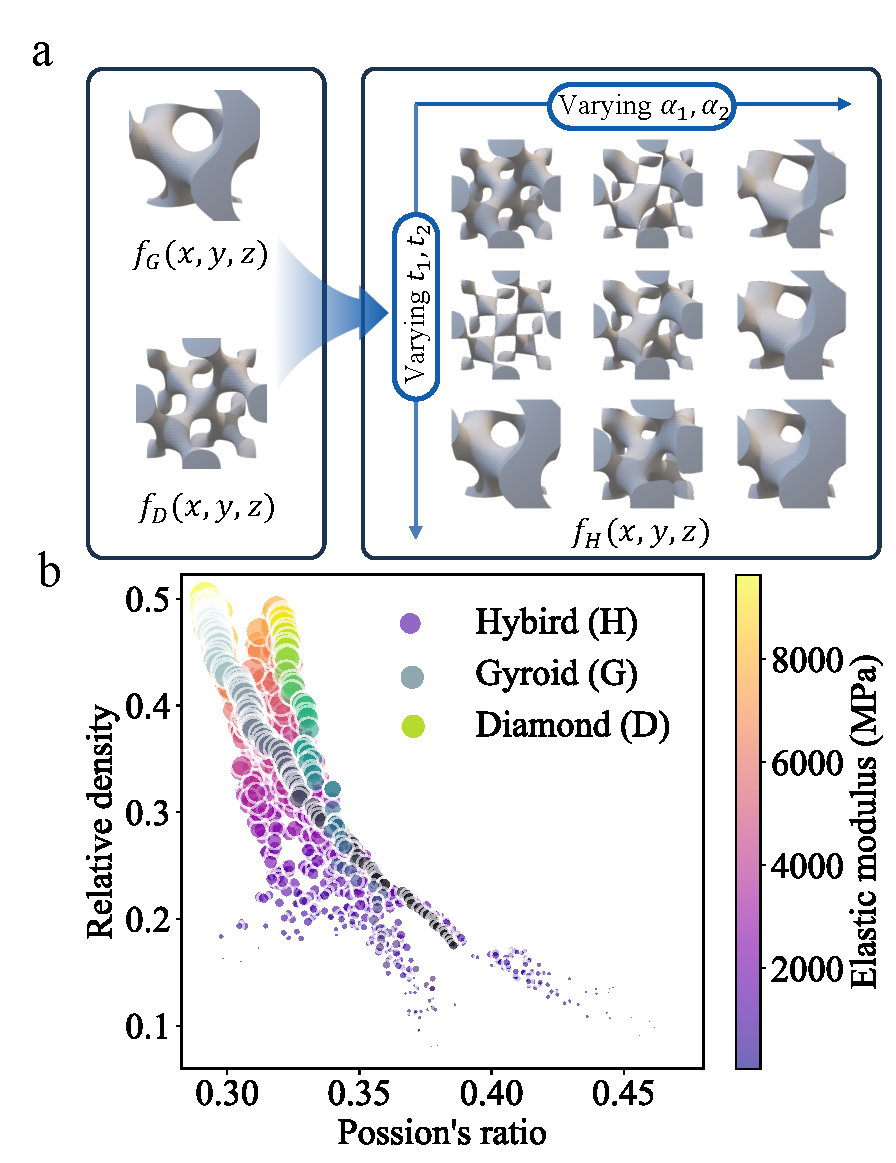
\includegraphics[width=0.75\linewidth]{figures/2.pdf}
    \caption{\textbf{Overview of the} \textbf{structure variation and} \textbf{property} \textbf{distribution} \textbf{of merged TPMS unit cells}. \textbf{a} Examples of different merged TPMS unit cell’s structure are realized by varying the shape parameters $\alpha_1, \alpha_2,t_1,t_2$ of Gyroid (G) and Diamond (D).\textbf{ b }The Effective elastic modulus $E$, Possion’s ratio $v$ and relative density $\rho$ in dataset (plasma colormap). The size of markers is proportional to $E$. Property variation of G and D structures with the increasing $t_i( i=1,2,\Delta t = 0.01$) within $f_G$ and $f_D$, each with a size of 100 are evaluated separately for comparison (bone and viridis colormap, respectively).}
    \label{fig:2}
\end{figure}  

\subsection{Performance of TPMS-WGAN}

To train a TPMS-GAN for generating a virtual design space with a target elastic modulus, we enable the elastic modulus condition while disabling other conditions in condition module. The database of hybrid TPMS unit cells is split with a ratio of 8:2 for training (1098) and testing (274), respectively. The coefficients $\alpha_1, \alpha_2$ of implicit function in database and the condition of elastic modulus $E$ are normalized before input to TPMS-GAN (more details are provided in Supplementary S4). We further improve the generative performance by ensuring the generated shape parameters can be accurately mapped back to their corresponding properties. Specially, we add a property navigator $R_\omega$ to predict the elastic modulus of each design. This lead to a additional loss terms:
\begin{equation}
\mathcal{L}_{(R_\omega)}=\mathbb{E}_{\boldsymbol{p}' \sim \mathbb{P}_g}(|R_\omega(\boldsymbol{p}')-E|)
\label{eq:18}
\end{equation}
Combining Eq. \ref{eq:7}, the final discriminator loss can be written by:
\begin{equation}
\mathcal{L}_{D_\theta} =  \mathcal{L}_{(G_\phi, D_\theta)} + \eta *\mathcal{L}_{R_\omega}
\label{eq:19}
\end{equation}
where $\eta$ is a hyperparameter set to 0.5, and the generator loss can be written by 
\begin{equation}
\mathcal{L}_{G_\phi} =  - \mathbb{E}_{\boldsymbol{z}\sim \mathcal{N}(\boldsymbol{0},\boldsymbol{I})} \left[ D_\theta (G_\phi(\boldsymbol{z}|\boldsymbol{C})\right]
\label{eq:20}
\end{equation}
Figure \ref{fig:4} provides a schematic comparison between the navigator-free TPMS-WGAN and the navigator TPMS-WGAN  (the hyper-parameters and architecture are provided in Supplementary Table S2). As depicted in Figure \ref{fig:4}a, the training loss of the navigator-generator, represented by the blue line, is more stable than that of the navigator-free generator, indicated by the green line. In WGAN, the discriminator's loss value serves as an indicator of model performance. Notably, the navigator discriminator exhibits a lower loss value of 2.57, compared to the navigator-free discriminator, which has a loss value of 3.12. Next, we use t-SNE and kernel smoothing function estimate (KSFE) based on the structure parameters of TPMS unit cell for the 2D visualization of the test data. As illustrated in Fig \ref{fig:4}c, d, the data distribution generated by the navigator generator more closely resembles the distribution of the training data compared to that produced by the navigator-free generator. To further assess the quality of the data generated by the navigator generator, we computed the Wasserstein distances \citep{Villani2008OptimalTO}. The results indicate a Wasserstein distance of \textbf{0.23} between the test data and the data generated by the navigator-free generator, and a distance of \textbf{0.34} between the test data and the data generated by the navigator generator. The diagonal plots of elastic modulus of test data and that evaluated of generated data of navigator-free generator and navigator generator via random forest model are shown in Fig \ref{fig:4}e, f (more details about random forest model as a surrogate model are provided in Supplementary S5). The elastic modulus of the structure generated by the navigator generator aligns more closely with the test data's elastic modulus than that produced by the navigator-free generator, with coefficients of determination ($R^2$) of 0.982 and 0.706, respectively. These results indicate that the navigator module effectively guides the gradient descent orientation of TPMS-GAN during training, enhancing its generative performance.

\begin{figure}
    \centering
    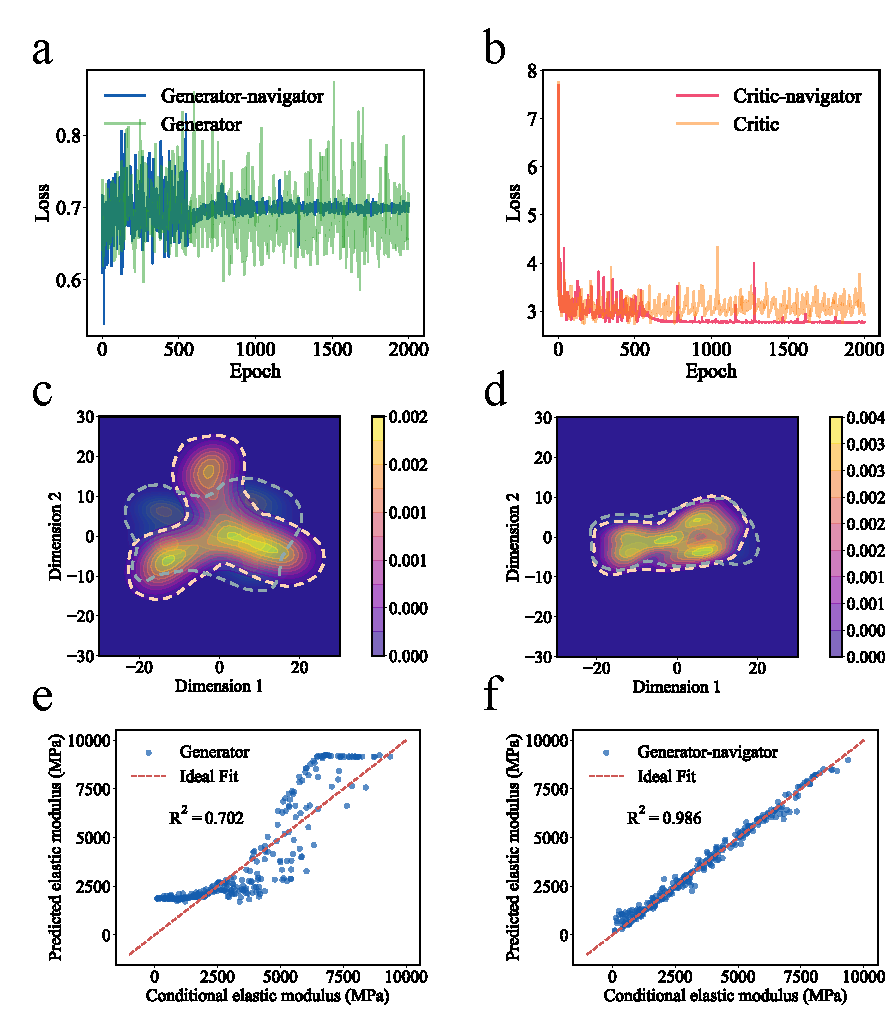
\includegraphics[width=0.75\linewidth]{figures/4.pdf}
    \caption{\textbf{Evaluation} \textbf{of} \textbf{the} \textbf{TPMS-GAN} \textbf{model. a} The loss value of navigator-free generator (green line) and navigator generator (blue line) during the training process. \textbf{b} The loss value of navigator-free discriminator (orange line) and navigator discriminator (red line) during the training process. The 2D t-SEN plot of training data distribution (viridis colormap) and generated data distribution (plasma colormap) under the corresponding elastic modules for navigator-free generator (\textbf{c}) and navigator generator (\textbf{d}), respectively. The density represents the probability estimate per unit area. The conditional elastic modulus and the evaluated elastic modulus of the generated structure of navigator-free generator (\textbf{e}) and navigator generator (\textbf{f})}.
    \label{fig:4}
\end{figure}

The continuous and low-dimensional latent space with generative cabilities is particularly advantageous for designing new structures by navigating this space through simple arithmetic operations on the latent representation $\boldsymbol{z}$. However, A general conditional WGAN lacks the ability to map a real structure to its latent space. To address the limitation, we trained an encoder, denoted as $IG_\psi$ to approximate inverse this mapping $(\boldsymbol{z},\boldsymbol{C})=IG_\psi(\boldsymbol{p})$. This inversion enables us to obtain a latent representation $\boldsymbol{z}$ from a real TPMS structure $\boldsymbol{p}$, facilitating exploration of the latent space through interpolation or variation. Although existing parameter-based and pixel/voxel-based generative models for cellular materials have successfully mapped topology and mechanical properties to a latent space using a similar data-driven design framework, they struggle to provide explainability in manipulating the geometry of TPMS unit cells via latent space or implicit function coefficients. By integrating a TPMS-GAN, once the latent representation $\boldsymbol{z}$ is obtained, explicit geometric control can be applied to a structure through geometric conditions. We term this framework Inversed TPMS-GAN (ITPMS-GAN). In this approach, the parameters $\boldsymbol{p}$ of the TPMS structure are encoded into a latent space $\boldsymbol{z}'$, together with the edited geometry condition $\bar{\boldsymbol{s}}$, serve as input into a well-trained generator. The generator then produces the parameters $\boldsymbol{p}'$ of the TPMS structure. Our methodology involves training the inverse mapping encoder $IG_\psi$ after the TPMS-GAN has been trained. To train $IG_\psi$, we utilize the structure parameters $\boldsymbol{p}$ of the TPMS unit cell and the generated parameters $\boldsymbol{p}'$ from the TPMS-GAN, minimizing a squared reconstruction loss $\mathcal{L}_{IG}$ (Fig \ref{fig:5}a).
\begin{equation}
    \mathcal{L}_{IG} = \frac{1}{m}\sum_{i=1}^m(\boldsymbol{p}^{(i)}-\boldsymbol{p}'^{(i)})= \frac{1}{m}\sum_{i=1}^m(\boldsymbol{p}^{(i)}-IG_\psi(\boldsymbol{z}',\bar{\boldsymbol{s}})^{(i)})
\label{eq:21}
\end{equation}
where $m$ is batch size, and the detail hyperparamenters and architecture of ITPMS-GAN are provided in Supplementary Table S4. A major advantage of ITPMS-GAN is its flexibility, allowing for explainable structural editing. As illustrated in Figure \ref{fig:5}b, the pore diameter of a TPMS unit cell from the test set can be edited using ITPMS-GAN. A TPMS unit cell, characterized by a relative density of\textbf{ 0.32 mm}, a pore diameter of \textbf{21 mm}, and a thickness of \textbf{14 mm}, is represented by a geometry vector $\boldsymbol{s}$ (Fig \ref{fig:5}b (iii)). To adjust the pore diameter in $\boldsymbol{s}$ to 19 mm, 20 mm, 21 mm, 22 mm, and 23 mm, we first map the structure parameters $\boldsymbol{p}$ to the latent representation $\boldsymbol{z}'$. This latent representation, combined with the specified pore diameter as a condition, serves as input to $G_\phi^2$ (more details about $G^2_\phi$ are provided in Supplementary Table S3). The generated TPMS structures exhibit a gradual variation corresponding to the variations of pore diameter, as depicted in Fig \ref{fig:5}b. We conducted simulations to assess the geometric characteristics of the generated structures. The actual geometries closely matched the designed ones, except for pore diameters of 19 mm and 23 mm, which measured 18.5 mm and 24 mm, respectively. In the 2D t-SNE plot of the training dataset structures (Fig \ref{fig:5}c), the generated structures are visualized to assess their spatial distribution. The structure with a pore diameter of 19 mm is located on the boundary of the TPMS structure, with the design error primarily resulting from the limited data available in the training set, hindering the model's ability to learn its features. Furthermore, there is a significant discrepancy between the pre-set and validated pore diameters for 23 mm and 24 mm. Figure \ref{fig:5}c also reveals that the structure \textbf{v} is positioned far from other designed structures, forming a distinct D-like shape, and exhibits greater similarity to structure G. The ITPMS-GAN model offers an explainable method for editing TPMS unit cells, instead of interpolation in latent space or adjusting implicit function coefficients. The approach can be applied to diverse structures in virtual design space or create a more refined design space.

\begin{figure}
    \centering
    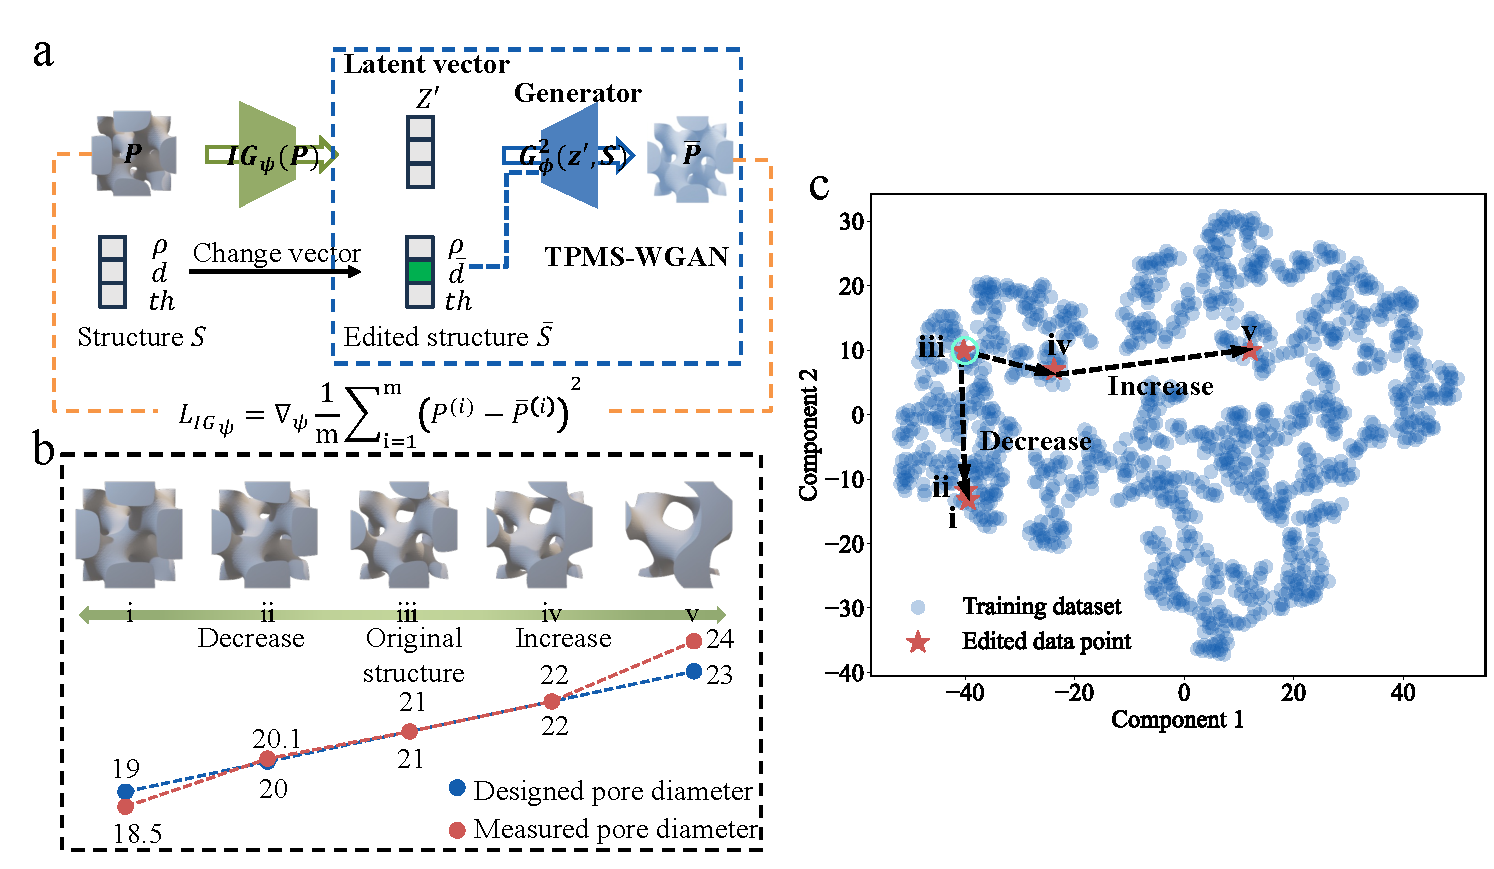
\includegraphics[width=1\linewidth]{figures/5.pdf}
    \caption{\textbf{Inversed TPMS-GAN (ITPMS-GAN) and representative examples of editing geometry of TPMS unit cells. a} The implicit function parameters $\boldsymbol{p}$ of TPMS unit cell with geometry features $\boldsymbol{s}$ is encode to latent vector $\boldsymbol{z}'$ by ITPMS-GAN, $IG_\psi$. And then the latent representation $\boldsymbol{z}'$ and the edited structure parameters $\bar{\boldsymbol{s}}$ are passed to generator $G_\phi^2$ to construct the TPMS unit cell. \textbf{b} The corresponding geometry evolution of TPMS unit cell is shown along the size variation of pore diameter. The designed pore diameters of TPMS unit cells by ITPMS-GAN are depicted as red dots, while the measured pore diameters are represented by blue dots. \textbf{c} The 2D t-SEN plot of implicit function parameters of training data (blue dots) and five designed TPMS unit cell (red stars). The structure evolution path of these five designed TPMS unit cells in the reduced parameters space of implicit function is shown by a black dashed line. }
    \label{fig:5}
\end{figure}

Bone is a typical cellular material primarily consisting of cortical and cancellous parts, with the elastic modulus ($E$) ranging from 30 to 30,000 MPa depending on the bone mineral density and varying according to age, sex, and race \citep{Wang2016}. Although bone can repair itself, a bone defect of a critical size necessitates a grafting implant to support the load and induce bone growth. For the application of TPMS unit cell in bio-implants, the two targets need to be optimized: (1) the $E$ of the scaffold implant must match that of the bone to relief stress shielding effect and frost the recovery of the bone \citep{Yang2020}. (2) the $\sigma_{ys}$ must be as high as possible to sustain the bone. 

In  the work, we employed the TPMS-GAN $G_\phi^1$ to generate 100,000 TPMS structures, forming a virtual design space $\Omega_E$ with a target elastic modulus of 6,000 MPa. As depicted in Figure \ref{fig:6}e, we compared the elastic modulus of these generated structures, as evaluated by a random forest model, with the pre-set value of 6,000 MPa (denoted by a red dashed line). The observed elastic modulus values ranged from 5,400 MPa to 6,300 MPa, clustering around the target modulus. To incorporate this target into constraint-aware active learning, we defined a constraint function based on the deviation of the generated structures' elastic modulus from the pre-set value of 6,000 MPa. This function is expressed as:
\begin{equation}
    c(\boldsymbol{p}') = 1 - \frac{|E(\boldsymbol{p}') - 6000|}{\max(|E(\boldsymbol{p}') - 6000|)}
\label{eq:22}
\end{equation}
The function $c(\boldsymbol{p}')$ reaches its maximum value when $E(\boldsymbol{p}') = 6000$. Figure \ref{fig:6}f illustrates the application of this constraint function within the virtual design space.

\begin{figure}
    \centering
    \includegraphics[width=0.75\linewidth]{figures/6.pdf}
    \caption{\textbf{Schematical figure of constrained-aware active learning strategy. a} The optimal value and predicted results with uncertainties in the cases of constraint-unaware (\textbf{a1}) and constraint-aware (\textbf{a2}). \textbf{b} The next query point according to EI (\textbf{b1}) and constrained-aware EI (\textbf{b2}). \textbf{c} The virtual design space of TPMS unit cell with a target elastic modulus of 6,000 MPa generate by generator $G_\phi^1$. \textbf{d} The application of elastic modulus constraint function within the virtual design space.}
    \label{fig:6}
\end{figure}

\subsection{Develop high yield strength TPMS unit cells with matched elastic modulus via the constraint-Aware Strategy}

The properties of the cellular materials are determined by both the scaffold architecture and the constituent materials. The mechanical response of the scaffold can be represented by a compressive stress-strain curve. Yield strength ($\sigma_{ys}$) is denoted by the yield point with 0.2 \% strain, which quantifies the maximum resistance prior to the onset of irreversible deformation. Calculating $\sigma_{ys}$ through simulation is resource-intensive due to the nonlinear plastic behavior of the constituent materials and the extensive number of discrete meshes involved. The yield strength calculation for each TPMS unit cell takes approximately 30 minutes, which is longer than the elastic modulus evaluation time of about 1 minute using FE simulation based on the numerical homogenization method (Details about computing platform are provided in Supplementary S6). BO method is efficiently to applied into expensive-to-evaluate black box problem. Here we propose an active learning approach to optimize yield strength while adhering to constraints on the elastic modulus. A support vector machine model is employed as the surrogate model, and bootstrap resampling is utilized to assess uncertainties by sampling the data with replacement. In present study, we sampled 16 candidates from the virtual design space and evaluated their yield strength using FEM. This process was repeated 50 times, generating 50 resampled training sets to construct 50 support vector machine models. Consequently, each sample in the initial dataset yields 50 predicted values, which are used to determine the mean value ($\mu$) and the associated standard deviation ($\Sigma$).

Figure \ref{fig:7}c illustrates the transition of the query sample from the blue dot to the red dot at the 1st iteration, facilitated by the elastic modulus constraint-aware EI approach introduced in \ref{sec:2-4}. This shift indicates that the constraint function of the elastic modulus alters the maximum expected improvement over the best observed value in the training dataset. A total of four iterations are performed, during which two samples are recommended and evaluated per iteration. The results are subsequently fed back into the dataset to initiate a new iteration.

The diagonal plot in Fig \ref{fig:7}a reveals that the model predictions are basically consistent with the observation values and the strategy of constraint-aware active learning recommended samples with high yield strength. We monitor mean square error (MSE) and R$^2$ as the surrogate model is successively refined with the results of evaluated TPMS structures  (Fig. \ref{fig:7}b). 

The elastic modulus and yield strength of all recommended samples are presented in Fig \ref{fig:7}(d,e,f). It is observed that the elastic modulus of these samples is closer to 6,000 MPa, with a mass center around 5,900 MPa, compared to the initial dataset, which has a mass center of approximately 5,800 MPa. Additionally, the yield strength of the recommended samples surpasses that of the initial dataset. To further demonstrate the efficacy of the constraint-aware active learning framework, the overall performance $Y$ of the TPMS unit cell is quantified by the following equation:

\begin{equation}
    Y = Y_E^N+Y_{\sigma_{ys}}^N
\label{eq:23}
\end{equation}
where 
\begin{equation}
    \begin{aligned}
    Y_E^N &= \frac{Y_E-\text{min}(Y_E)}{\text{max}(Y_E)-\text{min}(Y_E)} 
 ,Y_E = \frac{1}{|E(\boldsymbol{p}')-E^*|}\\
    Y^N_{\sigma_{ys}}& =\frac{Y_{\sigma_{ys}}-\text{min}(Y_{\sigma_{ys}})}{\text{max}(Y_{\sigma_{ys}})-\text{min}(Y_{\sigma_{ys}})} 
    \end{aligned}
\label{eq:24}
\end{equation}

This metric effectively reflects the design performance of TPMS unit cell in achieving a matched implant scaffold with enhanced yield strength. 


Figure \ref{fig:7}g indicates that the optimal structure was identified at the 2nd iteration, with a $Y$ value of 1.72, significantly higher than the optimal value of 0.22 in initial dataset. At the 3rd iteration, a decrease in overall performance was observed due to the active learning process, which integrates both exploration and exploitation capabilities. However, this approach led to improved performance at the 4th iteration. The stress-strain curve is depicted in Figure \ref{fig:7}i, while Figure \ref{fig:7}h presents the Von Mises' stress cloud plot. It is evident that stress concentration is localized at the junctions of unit cells. This study demonstrates that the constraint-aware active learning method successfully identified the optimal structure even beyond the training dataset, indicating a degree of extrapolation capability. Such robustness is particularly advantageous in clinical scenarios, where patient data, including target material properties and mechanical ranges, are often unknown in advance, and initial data distributions can vary widely. Furthermore, the design cost of TPMS unit cells with matched elastic modulus and high yield strength is significantly reduced by employing a method that requires the assessment of only 24 sample yield strengths. This is in stark contrast to the 1372 assessments needed in the one-step machine learning method used for training the generative model under bi-objective conditions. As a result, the design time is reduced about sixfold.

\begin{figure}
    \centering
    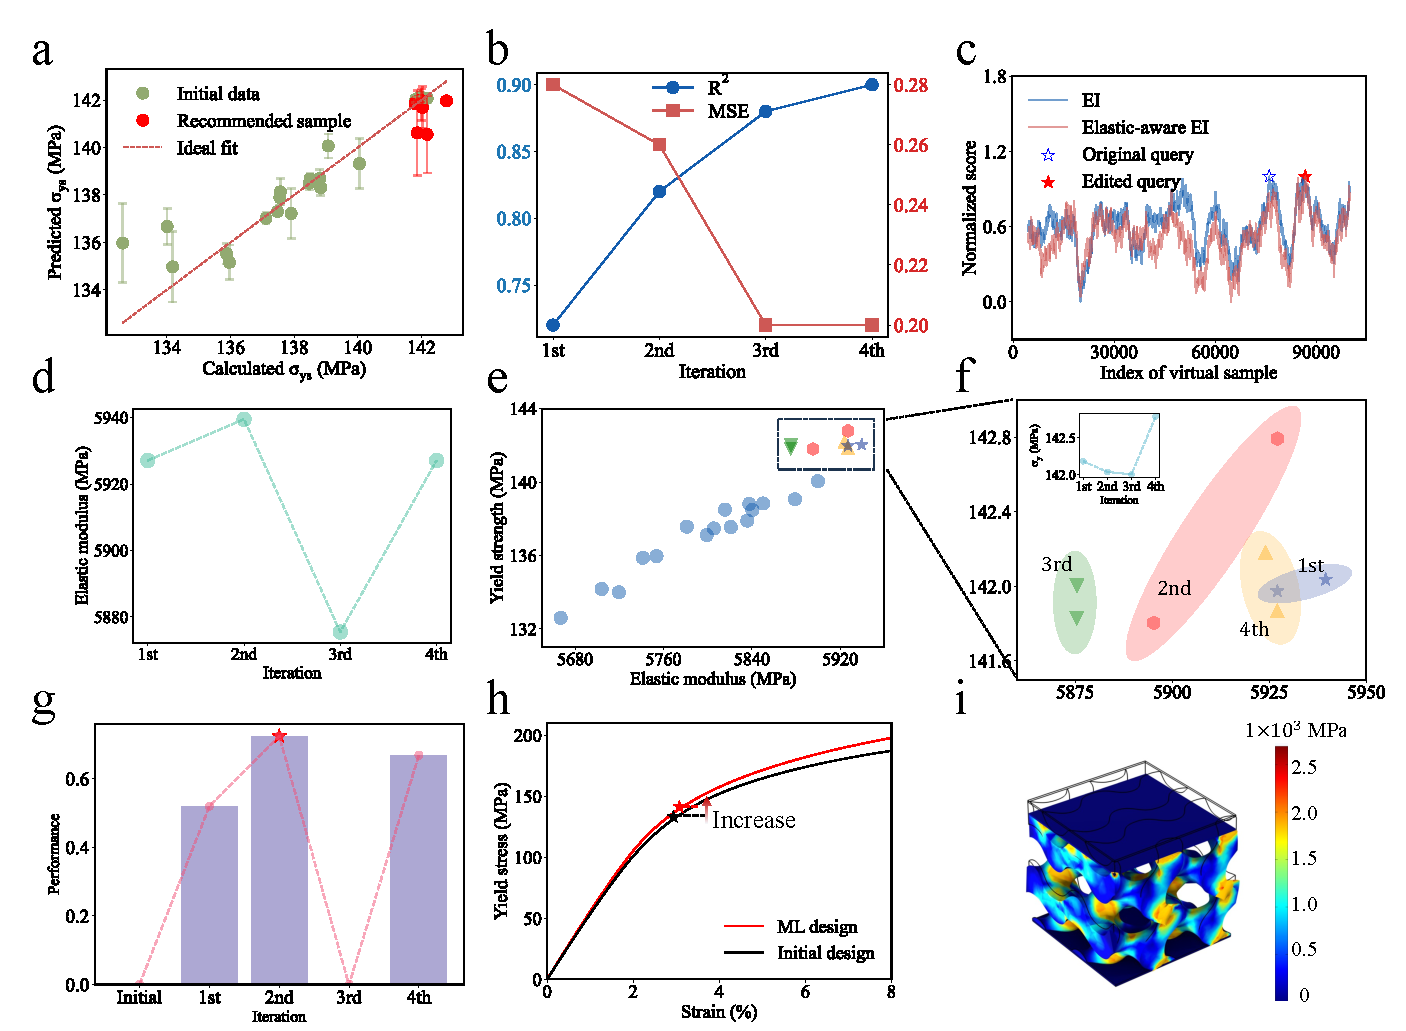
\includegraphics[width=1\linewidth]{figures/7.pdf}
    \caption{\textbf{Active learning workflow for yield stress of TPMS unit cells with elastic modulus constraint. a} Diagonal plot for SVM showing in red are the recommended structures and the green represents the initial data. \textbf{b} Performance of the SVM regressor as the iterations proceed. \textbf{c} Comparison of query points between EI and elastic modulus constraint-aware EI at 1st iteration. \textbf{d} Elastic modulus of the recommended structures as the iterations proceed. \textbf{e} The elastic modulus and yield strength distribution of recommended structures and the initial data (blue dots). \textbf{f} The elastic modulus and yield strength of recommended structures at each iteration of active learning. \textbf{g} The overall performance of TPMS unit cells as the iterations proceed. \textbf{h} The simulation strain-stress curves of the optimal structure recommended and the optimal 
structure in initial data. \textbf{g} The Von Mises' stress cloud plot of the optimal structure recommended in active learning.}
    \label{fig:7}
\end{figure}

\section{Conclusions}

In summary, a data-efficient two-stage bi-objective inverse design method of cellular materials based on TPMS is proposed, which combines generative model, active learning and FEM. The approach considers the unbalanced costs associated with different objectives. The cubic symmetric TPMS unit cells (G and D) were megred to create the rich dataset of isotropic cellular material in which the effective elastic tensor are calculated using a voxel-based numerical homogenization method. Our proposed TPMG-GAN with a navigator can generate the TPMS unit cells under desired conditions, here we generate TPMS unit cells under a target elastic modulus. The inversed TPMS-GAN also developed to  

% We proposed a GAN model to learn the IH mapping from properties to unit cell shapes that can be used to optimize functionally graded cellular structures. The cubic symmetric TPMS surfaces (P, D, and F-RD) were chosen and combined to create the dataset of isotropic cellular structures and represent each cellular unit cell as a six-dimensional shape vector (i.e., α1, α2, α3, t1, t2, t3). The unit cell property space consists of effective Young’s modulus, Poisson’s ratio, and relative density (i.e., E H , ν H , and ρ) in which E H and ν H were computed using a voxel-based numerical homogenization method. Our proposed IH-GAN’s one-to-many IH mapping was learned on the six-dimensional shape parameter space with the three-dimensional property space as the input conditions. Our approach offers an end-to-end generative model that automatically learns the IH mapping from data without assuming a bijective polynomial relationship. Except for the unit cell density (volume fraction), we also consider unit cell types when building the mapping. By including an auxiliary regressor in the IH-GAN, we can accurately generate the cellular unit cells that possess the desired properties (R2-scores between target properties and properties of generated unit cells > 98%). We also demonstrate the IH-GAN model’s efficacy by implementing it on modified structural optimization problems to construct multi-scale functionally graded cellular structures (e.g., a cantilever beam in this paper) using multiple types of cellular unit cells. Our approach addresses the connectivity issue between different types of unit cells simultaneously without a need for further compatibility optimization. By performing FE simulations, we validate that the beam constructed by IH-GAN improves the functional performance (e.g., 79.7% reduction in concentrated stress) compared to the conventional variable-density single-type beam structure. Moreover, the beam redesigned by IH-GAN can also achieve the target deformations with decent performance.


\section*{CRediT authorship contribution statement}
Jiaxuan Ma: Writing – original draft, Software, Methodology, Investigation, Formal analysis, Conceptualization. Bin Cao: Software, Investigation, Conceptualization, Formal analysis. Yuan Tian: Writing – review \& editing, Investigation, Formal analysis. Sheng Sun: Writing – review \& editing, Supervision, Funding acquisition, Formal analysis.

\section*{Declaration of competing interest}
The authors declare that they have no known competing financial interests or personal relationships that could have appeared
to influence the work reported in this paper.


%% The Appendices part is started with the command \appendix;
%% appendix sections are then done as normal sections
%% \appendix

%% \section{}
%% \label{}

%% If you have bibdatabase file and want bibtex to generate the
%% bibitems, please use
%%
\bibliographystyle{elsarticle-harv} 
\bibliography{refs}

%% else use the following coding to input the bibitems directly in the
%% TeX file.

% \begin{thebibliography}{00}

% %% \bibitem[Author(year)]{label}
% %% Text of bibliographic item

% \bibitem[ ()]{}

% \end{thebibliography}
\end{document}

\endinput
%%
%% End of file `elsarticle-template-harv.tex'.

